\documentclass{lecture}

%\setbeameroption{show notes on second screen}
\usepackage{listliketab}
\usepackage{url}
\usepackage{xspace}
\usepackage{graphicx}
\usepackage{LI}
\usepackage{etex}
\usepackage{booktabs}
\usepackage{color}
\usepackage{latexsym}
\usepackage{tipa}
%\usepackage{wasysym}
\usepackage{tipa}
\usepackage{tikz}
\usepackage{tikz-qtree}
%\usepackage{textpos}
%\usepackage{MnSymbol}
\usetikzlibrary{arrows,automata,calc,positioning,through}
%\usepackage{verbatim} % for comment blocks
%\usepackage{ulem} % for strikethrough (sout)
\usepackage{pifont}
%\usepackage{ucs}
\usepackage[utf8]{inputenc}
\usepackage[T1]{fontenc}
%\usepackage{pylistings}
\usepackage{amsmath}
\usepackage{multirow}


\usefonttheme{professionalfonts} % using non standard fonts for beamer
\usefonttheme{serif} % default family is serif
%\setmainfont{fourier}

\definecolor{darkgreen}{cmyk}{0.74,0.06,0.98,0.2}

\newcommand{\red}[1]{\textcolor{usydred}{#1}}
\newcommand{\green}[1]{\textcolor{darkgreen}{#1}}
\newcommand{\blue}[1]{\textcolor{usydblue}{#1}}
\newcommand{\gold}[1]{\textcolor{usydyellow}{#1}}

%\usepackage{beamerthemesplit}

%\usepackage{javalistings}
%\usepackage{cpplistings}
\beamertemplatenavigationsymbolsempty
%\setbeamertemplate{navigation symbols}{}
%\setbeamertemplate{bibliography item}[text]


\usepackage[style=authoryear]{biblatex}
\renewcommand*\bibopenparen{[}
\renewcommand*\bibcloseparen{]}
\addbibresource{slides.bib}

\title{A Practical Algorithm for Topic Modling with Provable Guarantees}
\author[Vanush \& Kristy]{Sanjeev Arora\\
		Rong Ge\\
		Yoni Halpern\\
		David Mimno\\
		Ankur Moitra\\
		David Sontag\\
		Yihcen Wu\\
		Michael Zhu}
\institute[\textschwa-lab]{Presented by: Vanush Vaswani and Kristy Hughes}
\date{}

\begin{document}

% Optional if you want to show outlines to structure the talk.
\AtBeginSection[]
{
  \begin{frame}
    %\frametitle{Outline: \thesection}
    \tableofcontents[currentsection]
  \end{frame}
}

\titleslide

%-------------------------------------------------%
\section[Intro]{Introduction}

\begin{plain}{Topic modeling}
	\begin{itemize}
		\p Statistical modeling
		\p Discovers hidden thematic structure (topics) in a collection of documents
		\p Help to develop new ways to:
		\begin{itemize}
			\p Search
			\p Browse
			\p Summarize
		\end{itemize}
	\end{itemize}
\end{plain}


\begin{plain}{Recent Work}
	\begin{itemize}
		\p Posterior inference is NP-hard (worst case)
		\p Approximate techniques used (SVD, Variational Inference, MCMC)
		\p Provably polynomial time algorithms: Statistical recovery problem
		\p Anandkumar et al. (2012)
			\begin{itemize}
				\p Third-order moments
				\p Assumes topics are not correlated
			\end{itemize}
		\p Arpra et al. 
			\begin{itemize}
				\p Second-order moments
				\p Assumes topics are separable 
				\p i.e. There exists an anchor word for every topic
				\p Steps: find anchor words, reconstruct topic distributions
			\end{itemize}
	\end{itemize}
\end{plain}

\begin{plain}{Contributions}
	\begin{itemize}
		\p Combinatorial anchor selection algorithm
			\begin{itemize}
				\p Assumes separability
				\p Stable in presence of noise
				\p Polynomial sample complexity
			\end{itemize}
		\p Simple probabilistic interpretation of the recovery step
			\begin{itemize}
				\p Arora et al. (2012) use matrix inversions $\rightarrow$ sensitive to noise
				\p Replace matrix inversion with gradient-based inference
			\end{itemize}
		\p Empirical comparison between recovery-based algorithms and existing likelihood-based algorithms
	\end{itemize}
\end{plain}


%------------------------------------------------%
\section[Background]{Background}

\begin{plain}{Modeling Process}
	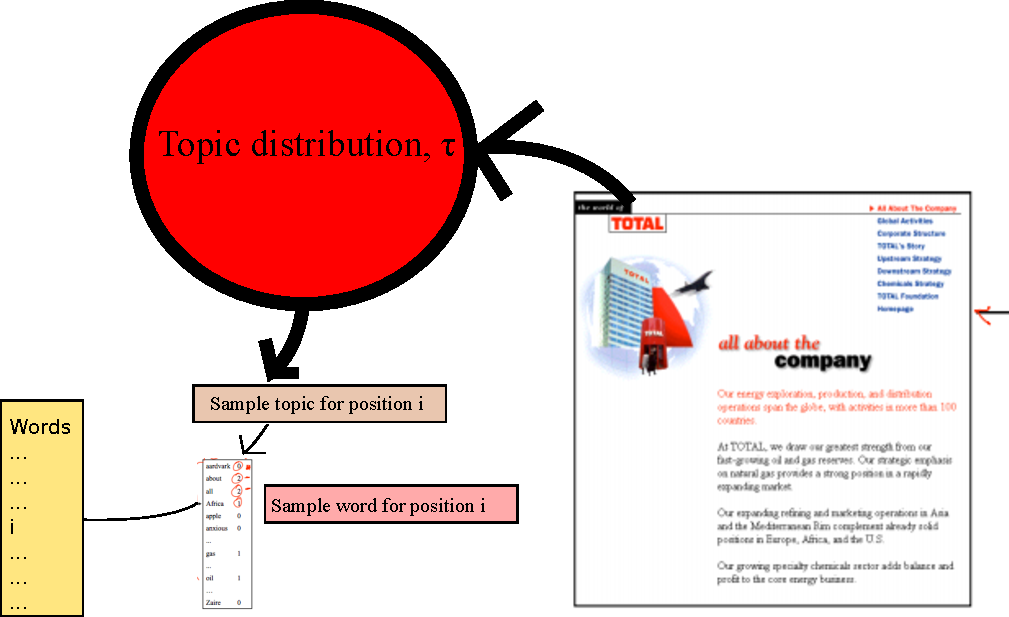
\includegraphics[scale=0.6]{figs/admixture}
\end{plain}

\begin{plain}{Task}
	\begin{itemize}
		\p Find the word-topic matrix, A
		\p Essentially statistical recovery
		\p Hyper-parameters of topic distribution
	\end{itemize}
\end{plain}

\begin{plain}{Word-topic matrix}
	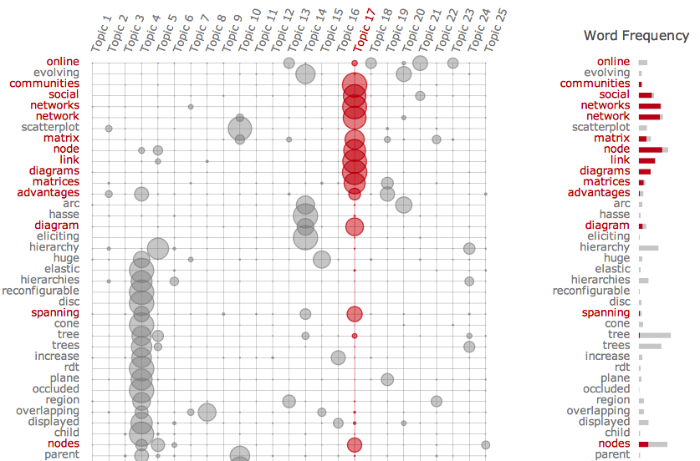
\includegraphics[scale=0.4]{figs/word_topic}
\end{plain}

%------------------------------------------------%
\section[Topic Recovery]{Topic Recovery via Bayes' Rule}

\begin{plain}{Mathematical Prerequisites}
	\begin{itemize}
		\p For each pair of words $w_1$ and $w_2$ 
		\p And their topic assignments $z_1$ and $z_2$
		\p The elements of the word-topic matrix are:\\
		$$A_{i,k} = p(w_1 = i | z_1 = k)$$
		\p Word co-occurrences:
		\begin{itemize}
			\p $Q \rightarrow$ joint probability of words occurring together
			\p $Q_{i,j} = p(w_1 = i, w_2 = j)$
			\p $\bar{Q}_{i,j} = p(w_2 = j | w_1 = i)$
		\end{itemize}
	\end{itemize}

\end{plain}

\begin{plain}{Convex Hulls}
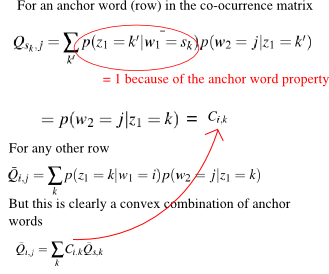
\includegraphics[scale=0.8]{figs/anchor_words}
\end{plain}

\begin{plain}{Convex Hulls}
\begin{center}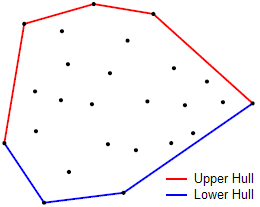
\includegraphics[scale = 0.6]{figs/convex_hull}\end{center}
Bayes Rule
$$p(w_1 = i | z_1 = k) = \frac{p(z_1 = k | w_1 = i)p(w_1 = i)}{\sum_i p(z_1 = k | w_1 = i^\prime)p(w_1 = i^\prime)}$$
\end{plain}


%------------------------------------------------------%
\section[Anchor Words]{Anchor Words}

\begin{plain}{Old algorithm}
\begin{center}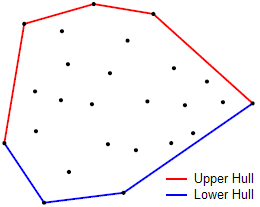
\includegraphics[scale = 0.6]{figs/convex_hull}\end{center}
Previous algorithm:\\
Anchor words $\rightarrow$ Vertices on convex hull\\
Use ILP to find vertices of hull $\rightarrow$ Inefficient
\end{plain}

\begin{plain}{New Algorithm}
	\begin{itemize}
		\p Iterative algorithm
		\begin{itemize}
			\p Finds farthest point from anchor words span
			\p This point becomes a new anchor word
		\end{itemize}
		\p New anchor words are most different from current anchor words
		\p Terminates after a set number of anchor words are found
	\end{itemize}
\end{plain}

%--------------------------------------------------%
\section[Results]{Experimental Results}
\begin{plain}{Methodology}
\end{plain}

\begin{plain}{Efficiency}
\end{plain}

\begin{plain}{Semi-synthetic documents}
\end{plain}

\begin{plain}{Real Documents}
\end{plain}


%---------------------------------------------------%
\section[Conclusion]{Conclusion}
\begin{plain}{Conclusion}
\end{plain}






\end{document}
